\documentclass[12pt]{article}
\usepackage{pgfplots}
\usepackage{graphicx}
\usepackage{float}
\begin{document}
\title{Statistics 12, Lab 1}
\date{January 22nd, 2019}
\author{Michael Wu\\UID: 404751542}
\maketitle

\section*{Section 1}

\subsection*{Problem 1}

\paragraph{a)}

The code ran with the following input and output.
\begin{verbatim}
> heights <- c(71, 68, 72)
> print(heights)
[1] 71 68 72
\end{verbatim}

\paragraph{b)}

The code ran with the following input and output.
\begin{verbatim}
> names <- c("Michael", "Hoang", "Huy")
> print(names)
[1] "Michael" "Hoang"   "Huy"
\end{verbatim}

\paragraph{c)}

The code ran with the following input and output.
\begin{verbatim}
> cbind(heights,names)
     heights names
[1,] "71"    "Michael"
[2,] "68"    "Hoang"
[3,] "72"    "Huy"
\end{verbatim}
The command created a matrix with the heights and names as column vectors, putting the heights in the left column
and the names in the right column. The class of this object is a matrix.

\subsection*{Problem 2}

\paragraph{a)}

I ran the following.
\begin{verbatim}
> NCbirths <- read.csv("births.csv")
\end{verbatim}

\paragraph{b)}

The code ran with the following input and output.
\scriptsize
\begin{verbatim}
> head(NCbirths)
  Gender Premie weight Apgar1 Fage Mage Feduc Meduc TotPreg Visits   Marital Racemom
1   Male     No    124      8   31   25    13    14       1     13   Married   White
2 Female     No    177      8   36   26     9    12       2     11 Unmarried   White
3   Male     No    107      3   30   16    12     8       2     10 Unmarried   White
4 Female     No    144      6   33   37    12    14       2     12 Unmarried   White
5   Male     No    117      9   36   33    10    16       2     19   Married   White
6 Female     No     98      4   31   29    14    16       3     20   Married   White
  Racedad Hispmom Hispdad Gained     Habit MomPriorCond BirthDef    DelivComp BirthComp
1   White NotHisp NotHisp     40 NonSmoker         None     None At Least One      None
2   White Mexican Mexican     20 NonSmoker         None     None At Least One      None
3 Unknown Mexican Unknown     70 NonSmoker At Least One     None At Least One      None
4   White NotHisp NotHisp     50 NonSmoker         None     None At Least One      None
5   Black NotHisp NotHisp     40 NonSmoker At Least One     None         None      None
6   White NotHisp NotHisp     21 NonSmoker         None     None         None      None
\end{verbatim}
\normalsize

\subsection*{Problem 3}

\paragraph{a)}

The code ran with the following input and output.
\begin{verbatim}
> find.package("maps")
[1] "C:/Users/chees/Documents/R/win-library/3.5/maps"
\end{verbatim}

\paragraph{b)}

I ran the following.
\begin{verbatim}
> map("state")
\end{verbatim}
The following plot was shown.
\begin{figure}[H]
    \begin{center}
        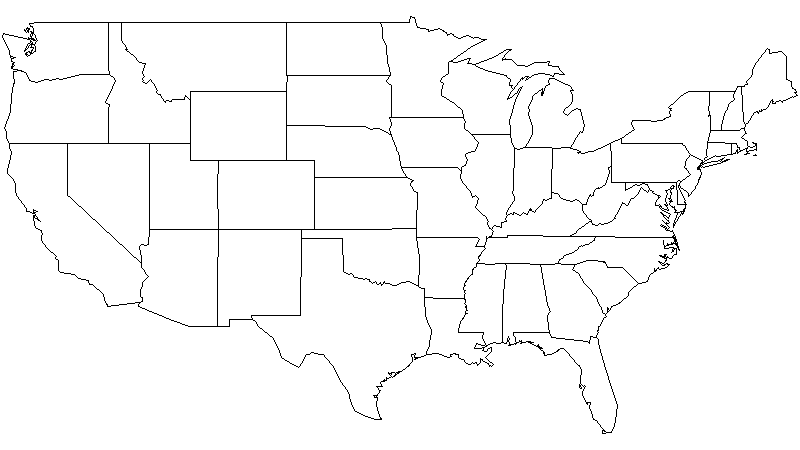
\includegraphics[width=4.5in]{section1problem3b.png}
    \end{center}
\end{figure}

\subsection*{Problem 4}

\paragraph{a)}

I ran the following.
\begin{verbatim}
> weights <- NCbirths$weight
\end{verbatim}

\paragraph{b)}

The weights are in ounces.

\paragraph{c)}

I ran the following.
\begin{verbatim}
> weights.in.pounds = weights/16
\end{verbatim}

\paragraph{d)}

The code ran with the following input and output.
\scriptsize
\begin{verbatim}
> weights.in.pounds[1:20]
 [1]  7.7500 11.0625  6.6875  9.0000  7.3125  6.1250  9.1875  8.6250  6.5000  7.6875
[11]  9.5625  8.0625  7.4375  6.7500  6.6250  7.8125  7.1875  8.0000  8.2500  5.1875
\end{verbatim}
\normalsize

\section*{Section 2}

\subsection*{Problem 1}

The code ran with the following input and output.
\begin{verbatim}
> mean(weights.in.pounds)
[1] 7.2532
\end{verbatim}

\subsection*{Problem 2}

The code ran with the following input and output.
\begin{verbatim}
> tally(NCbirths$Habit, "percent")
X
NonSmoker    Smoker
 90.61245   9.38755
\end{verbatim}

\subsection*{Problem 3}

The percentage of mothers who smoked was 11.61 percentage points lower than the percent of adult
Americans who smoked according to the CDC report.

\section*{Section 3}

\subsection*{Problem 1}

I ran the following.
\scriptsize
\begin{verbatim}
> dotPlot(weights.in.pounds, width=1, main="Birth Weights", xlab="Weight (lbs)")
\end{verbatim}
\normalsize
The following plot was shown.
\begin{figure}[H]
    \begin{center}
        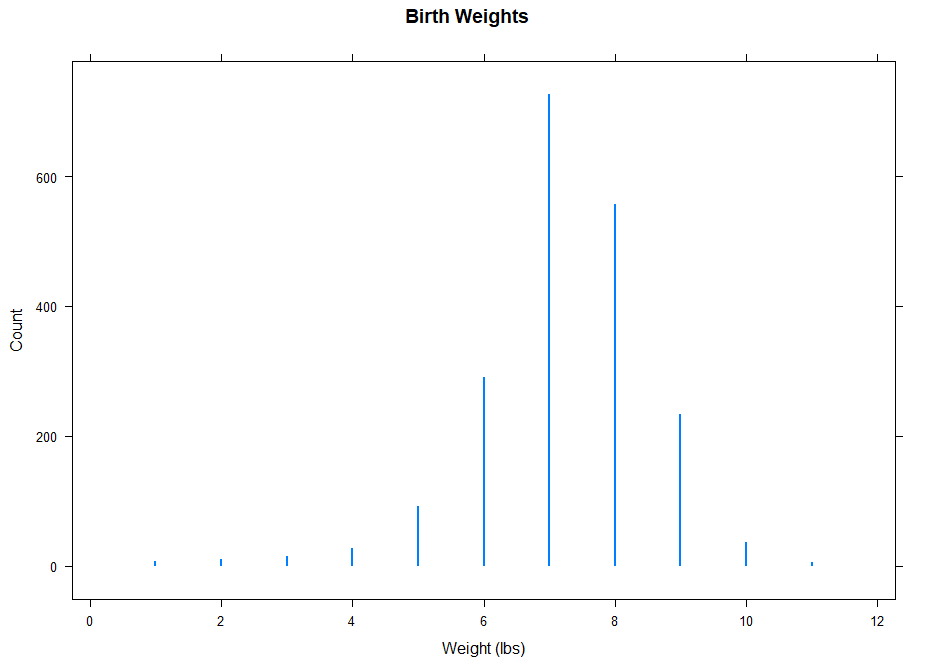
\includegraphics[width=3.5in]{section3problem1.png}
    \end{center}
\end{figure}

\subsection*{Problem 2}

I ran the following.
\scriptsize
\begin{verbatim}
> histogram(weights.in.pounds, nint=3, main="Birth Weights", xlab="Weight (lbs)")
> histogram(weights.in.pounds, nint=20, main="Birth Weights", xlab="Weight (lbs)")
> histogram(weights.in.pounds, nint=100, main="Birth Weights", xlab="Weight (lbs)")
\end{verbatim}
\normalsize
The following plots were shown.
\begin{figure}[H]
    \begin{center}
        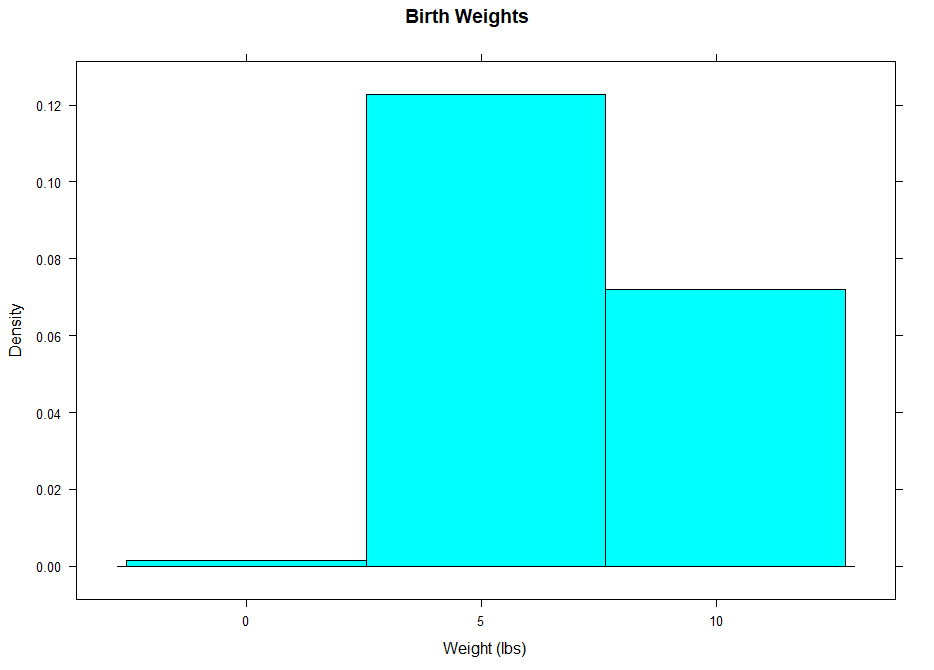
\includegraphics[width=3.5in]{section3problem2-3.png}
    \end{center}
\end{figure}
\begin{figure}[H]
    \begin{center}
        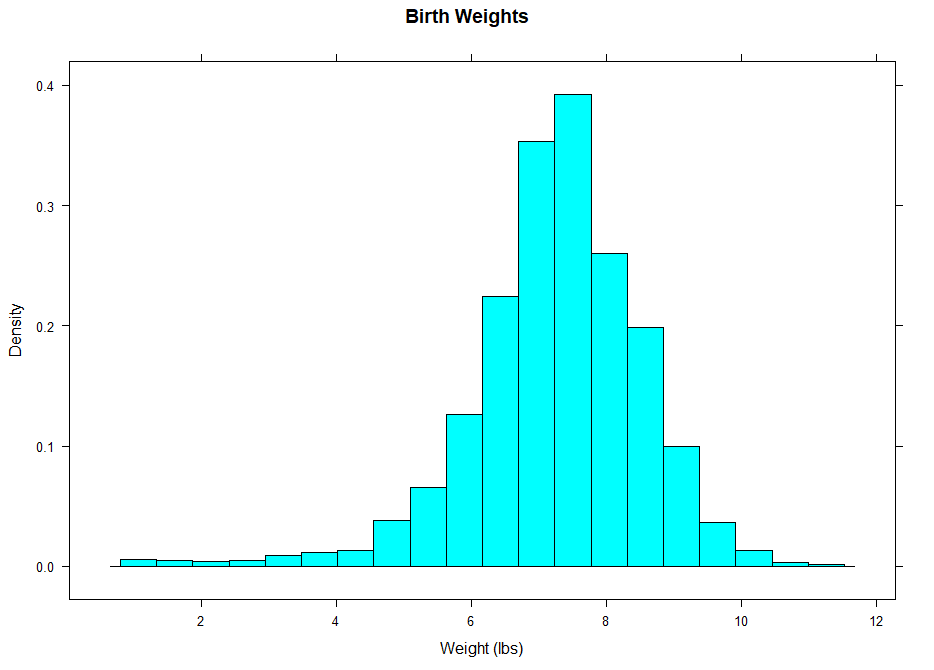
\includegraphics[width=3.5in]{section3problem2-20.png}
    \end{center}
\end{figure}
\begin{figure}[H]
    \begin{center}
        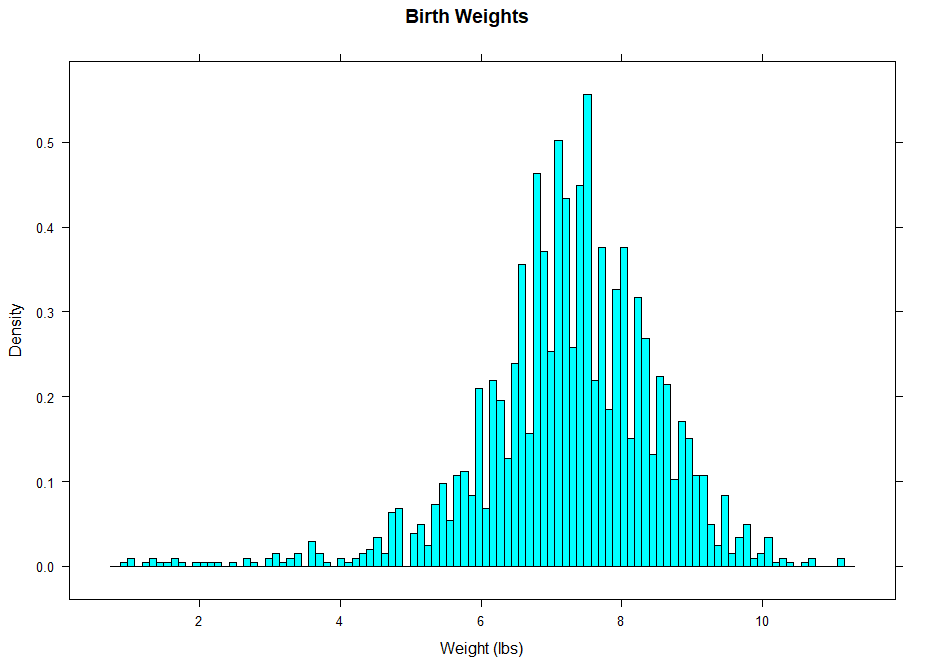
\includegraphics[width=3.5in]{section3problem2-100.png}
    \end{center}
\end{figure}
The histogram with 20 bins seems to give me the best visualization. The width of the bins is not too small so that it would lose detail
like with 3 bins, but it is not too high so that the plot would appear jagged like with 100 bins.

\subsection*{Problem 3}

I ran the following.
\tiny
\begin{verbatim}
> boxplot(NCbirths$Fage, NCbirths$Mage, main="Parent's Ages", names=c("Father's Age", "Mother's Age"))
\end{verbatim}
\normalsize
The following plot was shown.
\begin{figure}[H]
    \begin{center}
        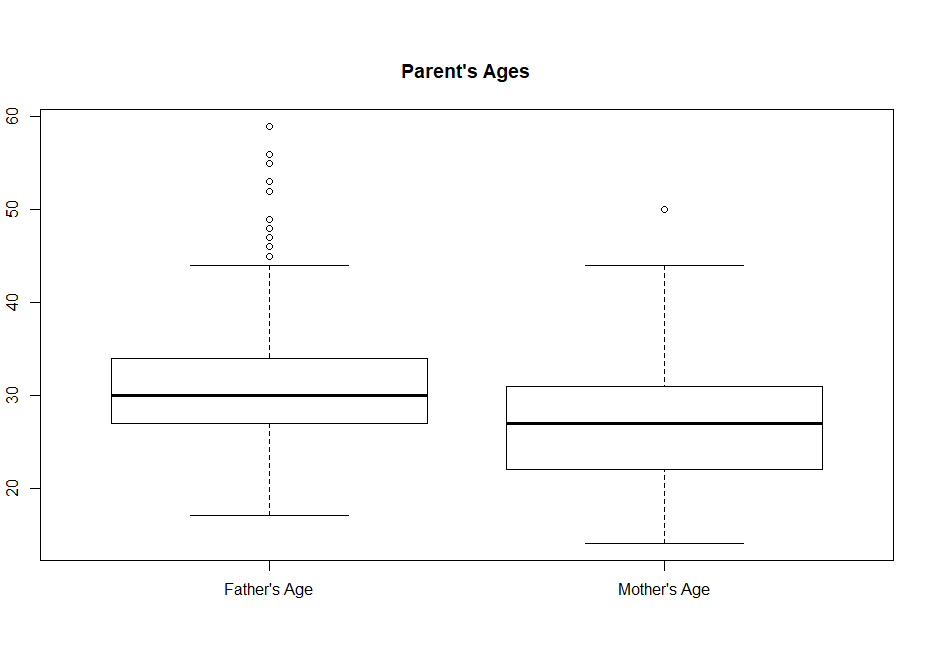
\includegraphics[width=3.5in]{section3problem3.png}
    \end{center}
\end{figure}
This plot shows that males tend to be older.

\subsection*{Problem 4}

I ran the following.
\scriptsize
\begin{verbatim}
> histogram(~weight | Habit, data = NCbirths, layout = c(1,2), width=10)
\end{verbatim}
\normalsize
The following plot was shown.
\begin{figure}[H]
    \begin{center}
        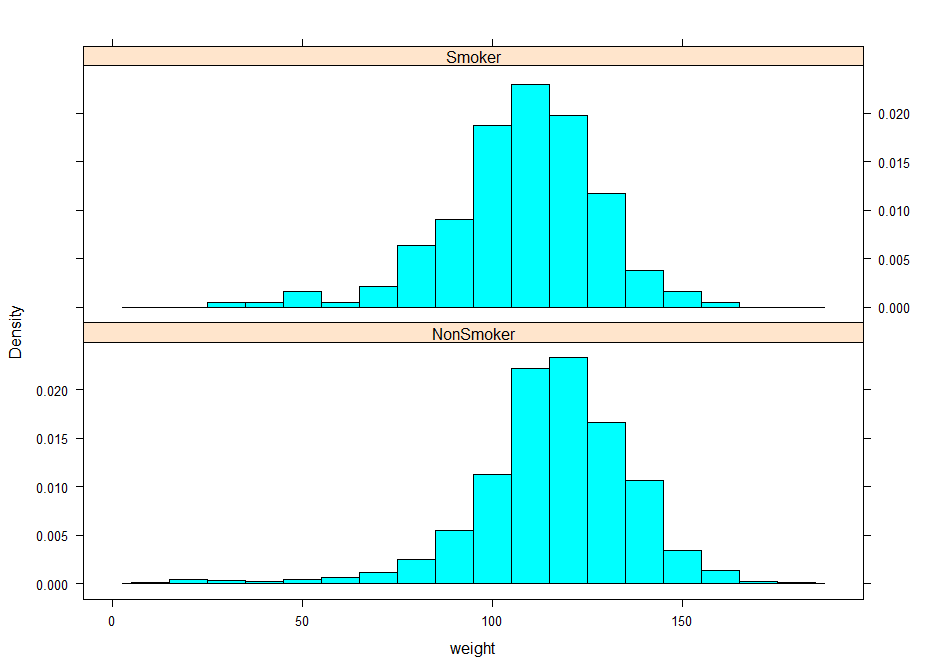
\includegraphics[width=3.5in]{section3problem4.png}
    \end{center}
\end{figure}
Average baby weights from mothers who smoke are slightly lower than average baby weights from mothers who do not smoke.

\section*{Section 4}

\subsection*{Problem 1}

Categorical variables related to the health of the baby that would be associated with the mother smoking would be prematurity,
birth defects, birth complications, and delivery complications. I ran the following code to output two way tables
to check my hypothesis.
\scriptsize
\begin{verbatim}
> tally(~Habit | Premie, data = NCbirths, format = "proportion")
           Premie
Habit               No        Yes
  NonSmoker 0.90889012 0.87845304
  Smoker    0.09110988 0.12154696

> tally(~Habit | BirthDef, data = NCbirths, format = "proportion")
           BirthDef
Habit       At Least One       None
  NonSmoker   0.80000000 0.90692969
  Smoker      0.20000000 0.09307031

> tally(~Habit | DelivComp, data = NCbirths, format = "proportion")
           DelivComp
Habit       At Least One      None
  NonSmoker    0.8920188 0.9127864
  Smoker       0.1079812 0.0872136

> tally(~Habit | BirthComp, data = NCbirths, format = "proportion")
           BirthComp
Habit       At Least One       None
  NonSmoker   0.86915888 0.90822281
  Smoker      0.13084112 0.09177719
\end{verbatim}
\normalsize
Here we can see that if a baby is born premature, the mother is a smoker 12.15\% of the time. If a baby is not born premature,
the mother is a smoker 9.11\% of the time. Thus smoking is associated with premature births. By comparing the given proportions
for birth defects, delivery complications, and birth complications, we can see that smoking is associated with all these variables
as well.

\section*{Section 5}

\subsection*{Problem 1}

I ran the following.
\scriptsize
\begin{verbatim}
> plot(weights.in.pounds ~ NCbirths$Mage, col="blue", cex = 0.5, pch = 19,
+      xlab = "Mother's age", ylab = "Baby weight (lbs)",
+      main = "Baby weight vs. Mother's age")
\end{verbatim}
\normalsize
The following plot was shown.
\begin{figure}[H]
    \begin{center}
        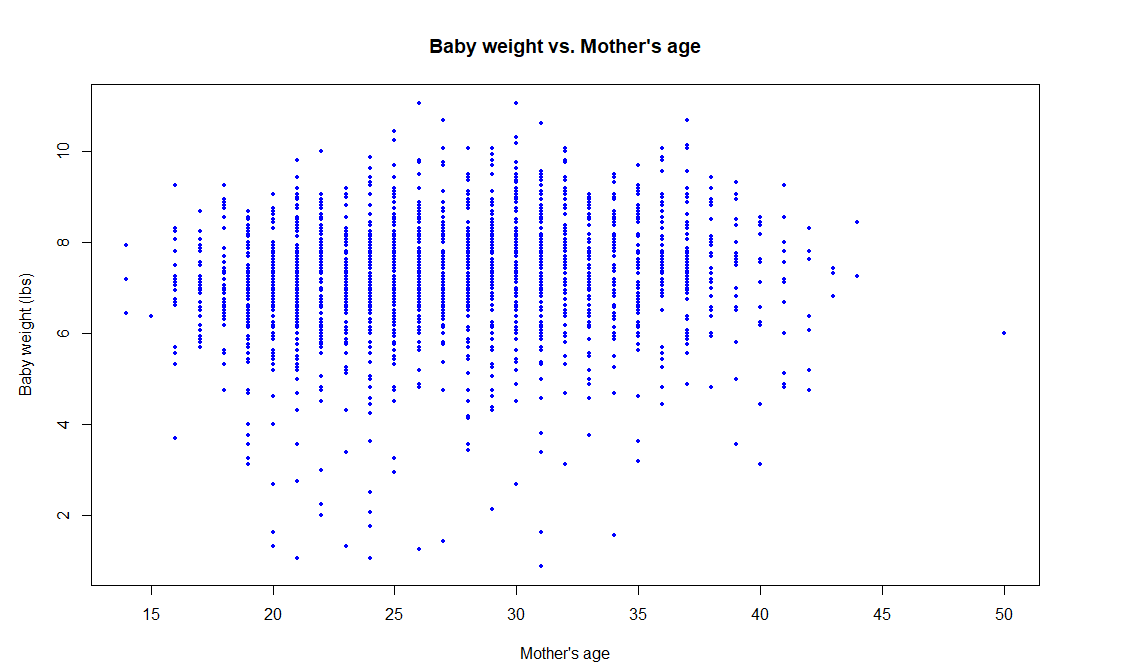
\includegraphics[width=5in]{section5problem1.png}
    \end{center}
\end{figure}

\section*{Section 6}

\subsection*{Problem 1}

I ran the following.
\scriptsize
\begin{verbatim}
> a <- read.table("http://www.stat.ucla.edu/~nchristo/statistics12/ozone.txt", header=TRUE)
> AQI_colors <- c("lightblue", "blue", "darkblue", "purple4", "black")
> AQI_levels <- cut(a$o3, c(0, 0.06, 0.075, 0.104, 0.115, 0.374))
> plot(a$x,a$y, xlim=c(-125,-114),ylim=c(32,43), xlab="Longitude",
+      ylab="Latitude", main="California ozone bubble plot", "n")
> map("county", "ca",add=TRUE)
> points(a$x,a$y, cex=a$o3/mean(a$o3),
+        col=AQI_colors[as.numeric(AQI_levels)], pch=18)
\end{verbatim}
\normalsize
The following plot was shown.
\begin{figure}[H]
    \begin{center}
        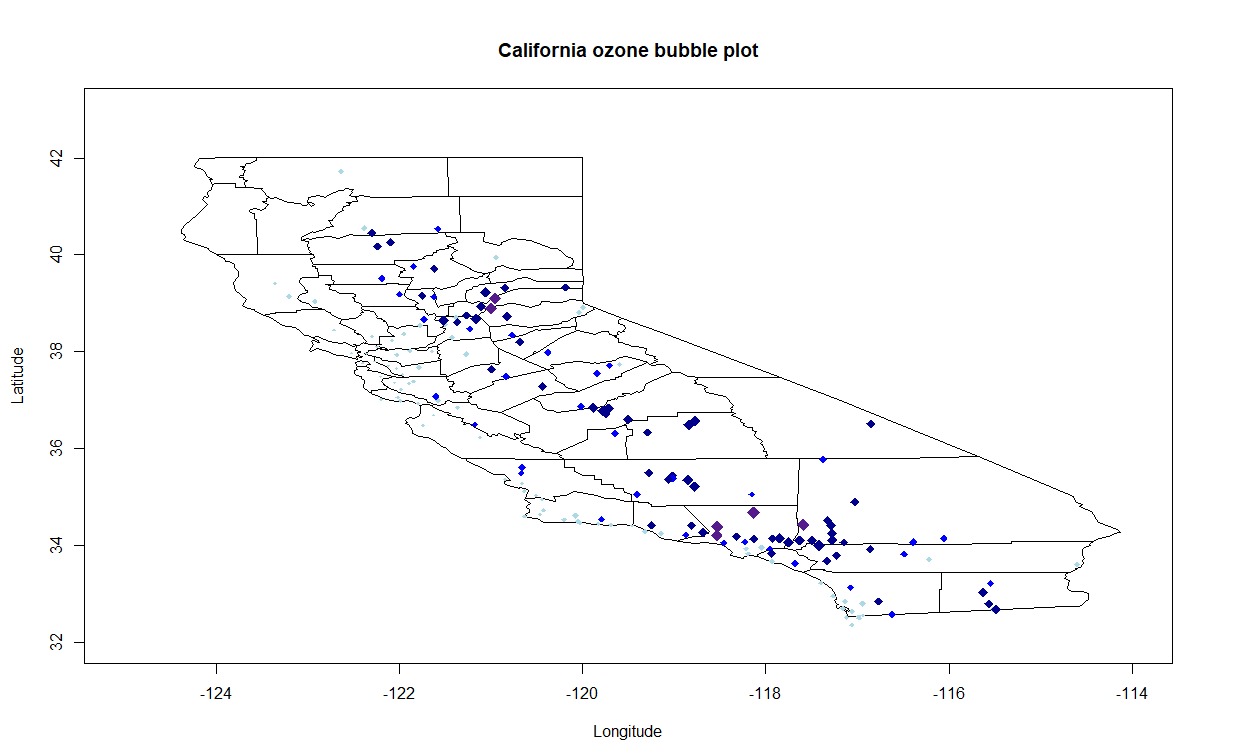
\includegraphics[width=5in]{section6problem1.png}
    \end{center}
\end{figure}

\end{document}